\documentclass[a4paper,12pt]{article} % тип документа


% Русский язык
\usepackage[T2A]{fontenc} % кодировка
\usepackage[utf8]{inputenc} % кодировка исходного текста
\usepackage[english,russian]{babel} % локализация и переносы


% Математика
\usepackage{amsmath,amsfonts,amssymb,amsthm,mathtools}


\usepackage{wasysym}

%Заговолок
\author{Талашкевич Даниил Александрович}

\title{Неделя 4. Графы I. Неориентированные графы}

\date{\today}

\begin{document}

\maketitle
\thispagestyle{empty}

\newpage
\setcounter{page}{1}
\begin{center}
\itshape
\bfseries
{ \Large Problems:}
\end{center}

\begin{center}
\section*{Задача 1}
\end{center}

Вершина степени $1$ соединена только с какой-то одной другой вершиной. Тогда должен существовать граф с $7$ вершинами и $22$ рёбрами.

Если граф полный, то количества его вершин равно $\frac{n\cdot (n-1)}{2} = \frac{7\cdot (7-1)}{2} = 21$. Значит при количестве вершин $7$ максимальное число ребёр достигается при полном графе и равно $21$, тогда рассматриваемого графа с $22$ вершинами не существует и условие не выполняется.

\begin{flushright}
\begin{large}
\textbf {Ответ: не выполняется}
\end{large}
\end{flushright}

\begin{center}
\section*{Задача 2}
\end{center}

Число, составленное из цифр-названий городов делится на $3$, если сумма этих цифр кратна 3.

Если цифра-название города кратна $3$, то она соединяется только с городами, чьи цифры-названия кратны 3. Значит города $3, 6$ и $9$ всегда соединены между собой и не соединены ни с какими другими городами. Тогда из $9$ можно попасть только в $3$ или $6$, а в $1$ попасть нельзя.

\begin{flushright}
\begin{large}
\textbf {Ответ: нельзя}
\end{large}
\end{flushright}
\newpage
\begin{center}
\section*{Задача 3}
\end{center}

Очевидно, что в любом несвязном графе существуют рёбра, не имеющие общий конец. Тогда рассмотрим только связные графы.

Пусть некоторая вершина $A$ соединяется с $n$ вершинами графа $X_i$ $(1 \leqslant i \leqslant n)$.

Если $n = 2$, то пусть вершины $X_1$ и $X_2$ соединены (другой случай см. в след. абзаце). При этом ни одна из трёх вершин $A, X_1, X_2$ не может быть соединена с какими-то другими вершинами: если существует какая-то вершина $Y$, соединённая с $X_i$ (или $A$) вершиной, то всегда найдётся ребро, не имеющее общий конец с ребром $Y-X_i$ $(Y-A)$ (особенно очевидно, если нарисовать рисунок). Получили граф-треугольник.

Если $n \geqslant 3$ и ни одна из вершин $X_i$ не соединена ни с одной другой, кроме $A$, то получим граф-звезду. Докажем, что других ситуаций в таком случае нет.

Пусть вершины $X_i$ и $X_j$ соединены, тогда как минимум рёбра $X_i-X_j$ и $X_{i+1}-A$ не имеют общий конец (если $i = n$, то вместо $i+1$ берём $1$), значит этот случай сразу отбрасываем.

Пусть вершины $X_i$ не соединены друг с другом, но в графе есть хотя бы одна вершина $B$, соединённая с какой-то вершиной $X_i$. Тогда, очевидно, можно взять ребро $X_j-X_k$ $(1 \leqslant j \leqslant n, 1 \leqslant k \leqslant n, i \neq j, i \neq k)$, которое не имеет общий конец с ребром $X_i-B$ -- такое ребро существует всегда при $n \geqslant 3$.

\underline{Итого получаем, что условиям удовлетворяют связные графы вида}\\ \underline{треугольник и звезда.}


\newpage
\begin{center}
\section*{Задача 4}
\end{center}

Цикл длины $3$ -- треугольник. Значит нужно доказать, что в графе с $400$ вершинами, где степень каждой равна $201$, есть хотя бы один треугольник.

Рассмотрим произвольную вершину графа $Y$. По условию она соединяется ещё с $201$ вершинами $X_i$ $(1 \leqslant i \leqslant 201)$. Предположим, что в рассматриваемом графе нет подграфа-треугольника. Значит вершины $X_i$ не могут быть соединены друг с другом, иначе образовался бы подграф-треугольник. Если $X_i$ не соединены друг с другом, то степень таких вершин максимум равняется $400-200 = 200$, но по условию степень всех вершин равна $201$, значит предположение о том, что вершины $X_i$ не соединены друг с другом неверно и существует хотя бы одно ребро $X_i-X_j$ $(x \neq j)$ -- образуется треугольник.

Значит из условий задачи следует, что существует хотя бы один цикл длины $3$.

\begin{flushright}
\begin{large}
\textbf {Доказано}
\end{large}
\end{flushright}


\begin{center}
\section*{Задача 5}
\end{center}

Если пересечение подграфов -- непустое множество, то существует хотя бы одна общая вершина для этих подграфов.

Пусть эта вершина -- единственная общая для двух подграфов, тогда она является пересечением этих графов. По определение граф является связным, если он содержит ровно одну компоненту связности -- между любой парой вершин существует по крайней мере $1$ путь. Значит для связности графа требуется хотя бы наличие одной пары вершин, что для пересечения рассматриваемых подграфов это не выполняется.

\begin{flushright}
\begin{large}
\textbf {Ответ: в общем случае неверно}
\end{large}
\end{flushright}
\newpage
\begin{center}
\section*{Задача 6}
\end{center}

С одного города можно попасть как минимум в $7$ других. Обозначим эти города $1, 2, ..., 8$. Подграф, состоящий из этих $8$ вершин -- связный.

Рассмотрим вершину графа, не рассмотренную ранее. Обозначим её $9$. Она связана как минимум с $7$ городами: либо только с городами 1-8, либо частично с $1-8$ и с $10-15$ (только с $10-15$ невозможно, так как это только 6 городов). То есть в любом случае город $9$ связан с каким-то из городов $1-8$, значит подграф $1-9$ -- связный.

Аналогично с вершиной $10$: она либо связана с вершинами $1-9$, либо частично с $1-9$ и частично с $11-15$, значит город $10$ связан с каким-то из $1-9$ и он -- связный.

Так продолжаем рассуждения до тех пор, пока не доберёмся до $15$ вершины. Она в любом случае связана с $1-14$ городами, значит подграф $1-15$ -- связный, а этот подграф и является исходным графом. Тогда из любого города можно добраться в любой другой город.

\begin{flushright}
\begin{large}
\textbf {Доказано}
\end{large}
\end{flushright}

\begin{center}
\section*{Задача 7}
\end{center}

Утверждение на языке теории графов: в каждом неориентированном графе существует две вершины одинаковой степени (если граф не пустой и не состоит из $1$-ой вершины).

Доказательство: пусть граф состоит из $n \geqslant 2$. Пусть у каждой вершины разная степень: $0, 1, 2, ..., n-1$. Значит должна существовать вершина со степенью $n-1$, то есть это вершина связана со всеми вершинами графа, но так как существует вершина со степенью $0$, которая не связана ни с одной вершиной, получаем противоречие.

\begin{flushright}
\begin{large}
\textbf {Доказано}
\end{large}
\end{flushright}

\newpage
\begin{center}
\section*{Задача 8}
\end{center}

Заметим, что у графа-цикла или графа-пути степень любой вершины равна $1$ или $2$. У дополнений этих графов степень вершин должна снова стать $1$ или $2$.

Пусть в графе $n$ вершин, если у вершины степень $1$ или $2$, то у дополнения графа у этой вершины степень равна $n-2$ или $n-3$. Максимальное число вершин графа реализуется при ситуации, когда у вершины дополнения графа степень $n-3$, а у графа степнь у этой же вершины $2$: $n-3 = 2 \Rightarrow n= 5$. Итак, в графе не более $5$ вершин.

Если $n=1$, то граф не является графом-циклом или графом-путём.

Если $n=2$, то дополнение графа -- изолированные друг от друга вершины.

Если $n= 3$, возможны $2$ ситуации: граф-путь $X_1-X_2-X_3$, тогда в его дополнеии вершина $X_2$ изолированна от остальных, и когда граф -- граф-цикл $X_1-X_2-X_3-X_1$, тогда дополнение графа -- $3$ изолированные вершины.

Если $n= 4$, возможны $2$ ситуации: граф-путь $X_1-X_2-X_3-X_4$, тогда его дополнение -- граф-путь $X_2-X_4-X_1-X_3$, и когда граф -- граф-цикл $X_1-X_2-X_3-X_4-X_1$, тогда дополнение графа -- объединение графов $X_1-X_4$ и $X_2-X_3$, что не удовлетворяет условиям.

Если $n= 5$, возможны $2$ ситуации: граф-путь $X_1-X_2-X_3-X_4-X_5$, тогда в его дополнении вершины $X_1$ и $X_5$ связаны двумя способами: напрямую $X_1-X_5$ и через вершину $X_3$: $X_1-X_3-X_5$, значит в дополнении графа содержится подграф-цикл, не равный самому графу -- не удовлетворяет условям. Вторая ситуация: граф-цикл $X_1-X_2-X_3-X_4-X_5-X_1$, тогда в дополнении графа степени вершин равны $5-2=3$, но из условий следует, как было написано раньше, что максимальная степень вершин -- $2$.

Подводя итоги, получаем следующие графы: \underline{граф-путь из $4$ вершин}
\underline{и граф-цикл из $5$ вершин}.

\newpage
\begin{center}
\section*{Задача 9}
\end{center}

Всего числа имею число разрядов $ = n$, тогда всего номеров будет $2\cdot 2\dots 2 =2^n$. Очевидно, что у нас число ребер $\frac{2^n}{2}$, так как любому числу $\dots 0110010\dots $ соответствует одно противоположное, где 1 заменены на 0 и наоборот. Тогда получаем, что 2 такие вершины создают одну компоненту связности и всего связных компонент будет  $\frac{2^n}{n}$.


\begin{flushright}
\begin{large}
\textbf {связных компонентов -- $\frac{2^n}{n}$}
\end{large}
\end{flushright}


\newpage
\begin{center}
\section*{Задача 10}
\end{center}

Примеры рисунков приведены ниже.

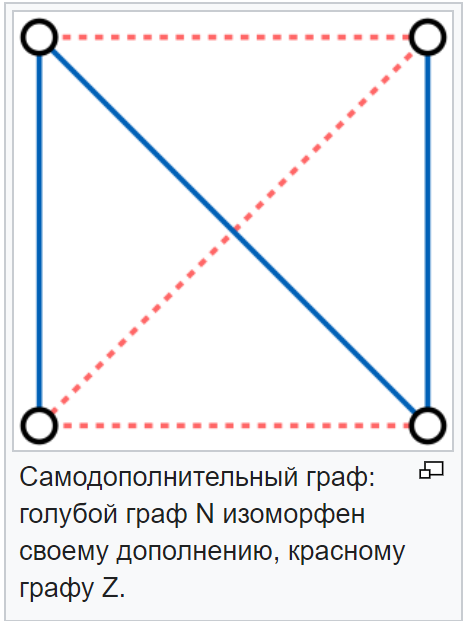
\includegraphics[width=\textwidth]{5 1}
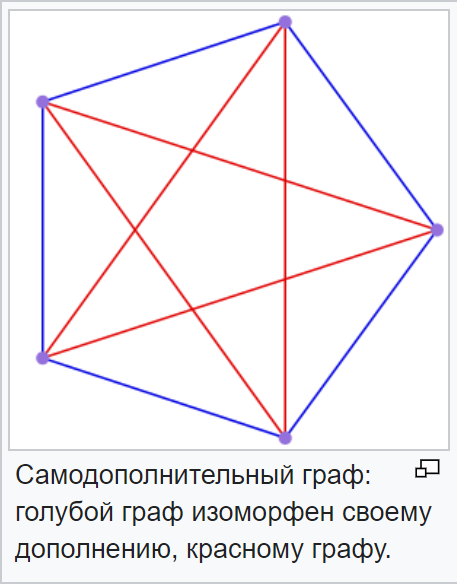
\includegraphics[width=\textwidth]{5 2}



\begin{flushright}
\begin{large}
\textbf {}
\end{large}
\end{flushright}


 \end{document}
